\documentclass{article}
\usepackage{tikz}
\usepackage{blindtext}
\usetikzlibrary{automata,positioning,arrows}
\usepackage[T1]{fontenc}
\usepackage{hyperref}
\usepackage{graphicx}
\graphicspath{.}

\title{EECS 510 Final Project}
\author{Jack Bauer}
\date{December 2024}

\begin{document}

\maketitle
\section{Part 1 - Design a Formal Language}
Inspired by some of my favorite novels, I have designed a language based on spell-casting. Spells consist of some combination of these four elements: fire, earth, air, and water. However, for any aspiring mage, there are three main rules to be aware of:
\begin{enumerate}
    \item 
    Fire and water are opposites, and as such they cannot appear next to each other in a valid spell. Earth and air are also opposites; they cannot appear next to each other either. 
    \item 
    Fire and earth make up the dark side. Air and water form the light side. However, light and dark must always be in balance, so there must be an equal number of light and dark elements; that is, an equal number of occurrences of fire/earth and air/water in any valid spell.
    \item 
    After extensive study, the Mages' Guild has discovered that, as fire and earth are the most foundational elements, they must come first in any valid spell.
    \item
    Finally, nothing is not a valid spell. There's no magic in the absence of magic, right? 
\end{enumerate}
For more details, see below. Fire is represented as f, air as a, water as w, and earth as e. If you learn these rules, you will become more powerful than you can imagine!
\begin{center}
    $\Sigma$ = \{f, e, a, w\}\\
    $\Gamma$ = \{X\} \\
    \hfill \\ 
\end{center}
Rules
\begin{itemize}
    \item f and w cannot follow each other.
    \item a and e cannot follow each other.
    \item D = \{f, e\} and L = \{a, w\}. There must be an equal number of elements from L and D. 
    \item All elements from D must precede all elements from L. 
    \item $\lambda$ is not a valid string.
    \end{itemize}
Some example strings: fffeeewaaawaw, fa, ew, eefewaaw.
\section{Part 2 - Grammar}
The grammar of this language is context-free. It is as follows:
\begin{center}
    $S\rightarrow$ T | DSL \\
    $L\rightarrow$ a | w\\
    $D \rightarrow$ f | e \\
    $T \rightarrow$ fa | ew
\end{center}
\section{Part 3 - Automaton}
Definitions: 
\begin{center}
    \begin{itemize}
        \item Q = \{$q_s$, $q_f$, $q_e$, $q_a$, $q_w$\}
        \item $\delta$ =\\ $\{
        ((q_s,f, \lambda), (q_f,X)),
        ((q_s,e, \lambda), (q_e,X)),$\\
        $((q_f,f, \lambda), (q_f,X)),
        ((q_f,a, X), (q_a,\lambda)),
        ((q_f,e, \lambda), (q_e,X))$\\
        $((q_e,e, \lambda), (q_e,X)),
        ((q_e,w, X), (q_w,\lambda)),
        ((q_e,f, \lambda), (q_f,X)),$\\
        $((q_w,a, X), (q_a,\lambda)),
        ((q_w,w, X), (q_w,\lambda)),$\\
        $((q_a,a, X), (q_a,\lambda)),
        ((q_a,w, X), (q_w,\lambda))
        \}$
    \end{itemize}
\end{center}
For the PDA, see Figure 1. 
\begin{figure}
    \centering
    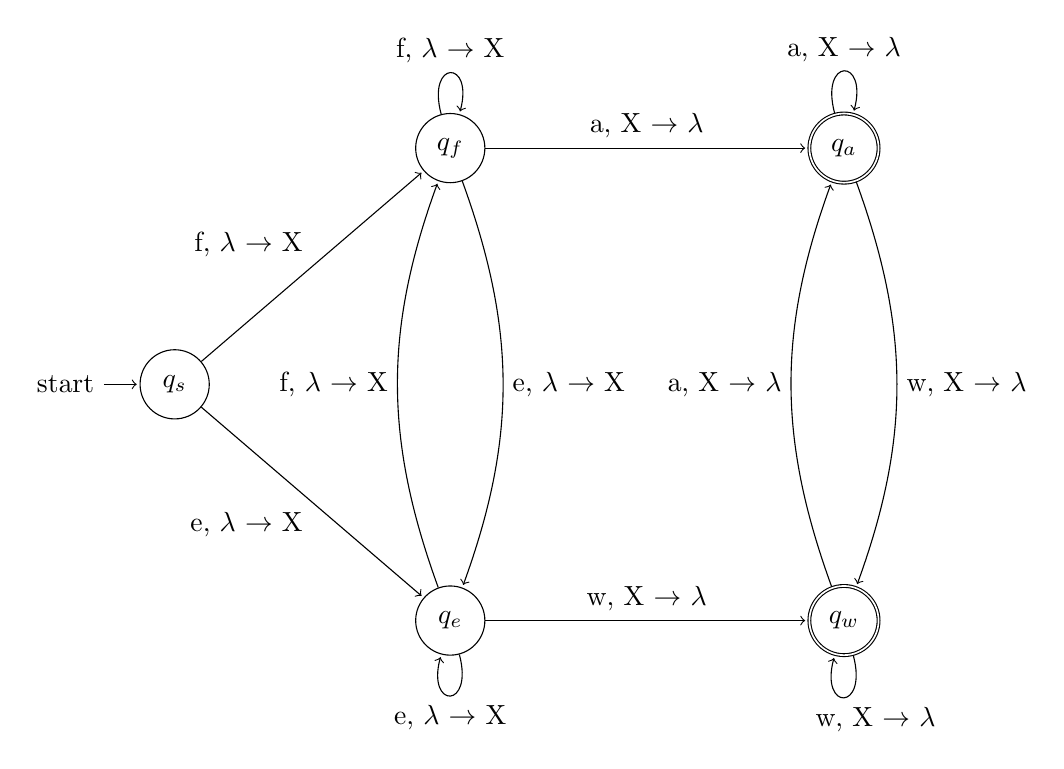
\begin{tikzpicture}[shorten >= 1pt, node distance=2cm,on grid,auto]
    \node[state,initial] (q_s) at (-5.5, 0) {$q_s$};
    \node[state] (q_f) at (-2, 3) {$q_f$};
    \node[state,accepting] (q_a) at (3, 3) {$q_a$};
    \node[state,accepting] (q_w) at (3, -3) {$q_w$};
    \node[state] (q_e) at (-2, -3) {$q_e$};
    \path[->]
    (q_s) edge node {f, $\lambda$ $\rightarrow$ X} (q_f)
          %edge [bend right=80, looseness=1.5] node [swap] {W, $\lambda$ $\rightarrow$ L} (q_w)
          %edge node [swap] {A, $\lambda$ $\rightarrow$ L} (q_a)
          edge [swap] node {e, $\lambda$ $\rightarrow$ X} (q_e)
    (q_f) %edge [loop above] node {F, L $\rightarrow$ D} ()
          edge [loop above] node [] {f, $\lambda$ $\rightarrow$ X} ()
          %edge [bend left=20] node {E, L $\rightarrow$ D} (q_e)
          edge [bend left=20] node {e, $\lambda$ $\rightarrow$ X} (q_e)
          edge node {a, X $\rightarrow$ $\lambda$} (q_a)
          %edge [bend left=20] node [yshift=-.4cm] {A, $\lambda$ $\rightarrow$ L} (q_a)
    (q_e) %edge [loop below] node {E, L $\rightarrow$ D} ()
          edge [loop below] node {e, $\lambda$ $\rightarrow$ X} ()
          %edge [bend left=20] node {E, L $\rightarrow$ D} (q_f)
          edge [bend left=20] node {f, $\lambda$ $\rightarrow$ X} (q_f)
          edge node {w, X $\rightarrow$ $\lambda$} (q_w)
          %edge [] node [yshift=-.4cm] {W, $\lambda$ $\rightarrow$ L} (q_w)
    (q_w) edge [loop below] node [xshift=.4cm] {w, X $\rightarrow$ $\lambda$} ()
          %edge [loop below] node [below=of q_w, yshift=1.3cm, xshift=.4cm] {W, $\lambda$ $\rightarrow$ L} ()
          edge [bend left=20] node {a, X $\rightarrow$ $\lambda$} (q_a)
          %edge [bend left=20] node [yshift=-.4cm] {A, $\lambda$ $\rightarrow$ L} (q_a)
          %edge [bend left=20] node {E, L $\rightarrow$ D} (q_e)
          %edge [bend left=20] node [yshift=-.4cm] {E, $\lambda$ $\rightarrow$ D} (q_e)
    (q_a) edge [loop above] node {a, X $\rightarrow$ $\lambda$} ()
          %edge [loop below] node [below=of q_a, yshift=1.3cm] {A, $\lambda$ $\rightarrow$ L} ()
          edge [bend left=20] node {w, X $\rightarrow$ $\lambda$} (q_w);
          %edge [bend left=20] node [yshift=.4cm] {W, $\lambda$ $\rightarrow$ L} (q_w)
          %edge [bend left=20] node {F, L $\rightarrow$ D} (q_f)
          %edge [bend left=20] node [yshift=-.4cm] {F, $\lambda$ $\rightarrow$ D} (q_f);
    \end{tikzpicture}
    \caption{PDA for the Elemental Language}
    \label{fig:enter-label}
\end{figure}
\newpage
\section{Part 4 - Data Structure}
The data structure for this language is stored as a file in memory. The file format is as follows:\\
- Line 1: A whitespace-delimited list of states.\\
- Line 2: A whitespace-delimited list of input symbols. \\
- Line 3: A whitespace-delimited list of stack symbols. \\
- Line 4: The start state. \\
- Line 5: A whitespace-delimited list of accepting states. \\
- Lines 6-17: Each line is a whitespace-delimited list of elements representing a transition, in the following order:
\begin{enumerate}
    \item The beginning state of the transition.
    \item The input character.
    \item The ending state of the transition.
    \item The stack variable popped. An \_ represents $\lambda$.
    \item The stack variable pushed. An \_ represents $\lambda$. 
\end{enumerate}
Using this format, the automaton can be represented as a text file with the following 17 lines:
\begin{enumerate}
    \item q\_s q\_f q\_e q\_w q\_a
    \item a e f w
    \item X
    \item q\_s
    \item q\_a q\_w
    \item q\_s f q\_f \_ X
    \item q\_s e q\_e \_ X
    \item q\_f f q\_f \_ X
    \item q\_f e q\_e \_ X
    \item q\_f a q\_a X \_
    \item q\_e f q\_f \_ X
    \item q\_e e q\_e \_ X
    \item q\_e w q\_w X \_
    \item q\_a a q\_a X \_
    \item q\_a w q\_w X \_
    \item q\_w a q\_a X \_
    \item q\_w w q\_w X \_
\end{enumerate}

\section{Part 5 - Testing}
The code to test strings for the automaton is located here:
\url{https://github.com/bribedjupiter/eecs510_final_project}. There is a file, main.py, that when ran will ask the user for an input string. It will then load the automaton from automaton.txt, represented using the data structure from Part 4, and then call a function to check if the automaton accepts the input string. If it accepts, then it will list the steps it took while processing the string. If it rejects, it will simply say reject. It is also possible that it may raise an error, but if it does it may be the result of a malformed input file. Here is a sample output:
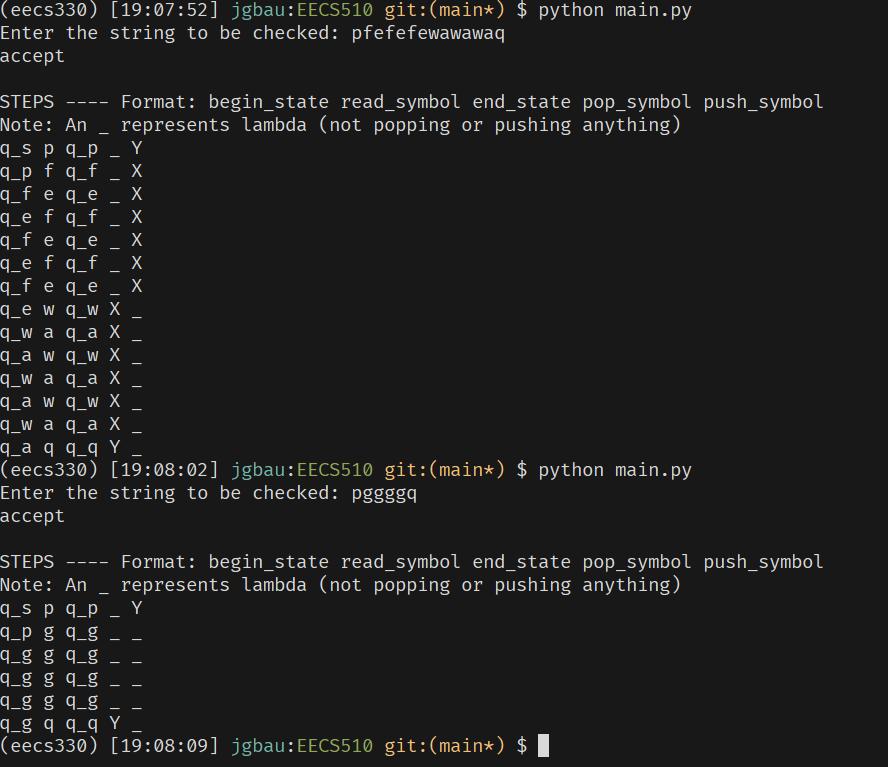
\includegraphics[width=\textwidth]{part5-accept.png}
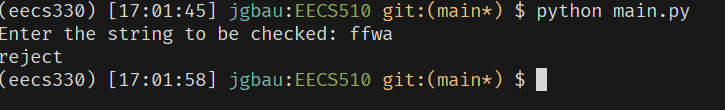
\includegraphics[width=\textwidth]{part5-reject.png}
\end{document}
